\documentclass[14pt]{beamer}

\title[NST]{Neural Style Transfer}
\subtitle{NeuralArt - Stylize your Image}
\author[Team - 38]{Avishi Gupta, Vaseem Naazleen, Shivangi Tomar}
\date{18 July 2020}

\usetheme{Madrid}
\usepackage{graphicx}

\begin{document}

\begin{frame}
   \titlepage
\end{frame}

\begin{frame}
		\frametitle{Overview}
		Our project aims to stylize image by implementing A Neural Algorithm of Artistic Style paper by Leon A. Gatys, Alexander S. Ecker and Matthias Bethge. \\~\\

		https://arxiv.org/pdf/1508.06576.pdf
\end{frame}

\begin{frame}
		\frametitle{What is Neural Style Transfer?}
		\setbeamertemplate{itemize items}[ball]
		\begin{itemize}
            \item Neural Style Transfer is an optimization technique.
           \item Input:
		\begin{itemize}
		     \item Content image
		     \item Style reference image
		\end{itemize}
             \item Output:
		\begin{itemize}
             \item Stylized image: looks like the content image, but \say{painted} in the style of the style
        reference image
        \end{itemize}
        \end{itemize}
\end{frame}

\begin{frame}
    \frametitle{Example}
    \begin{center}
        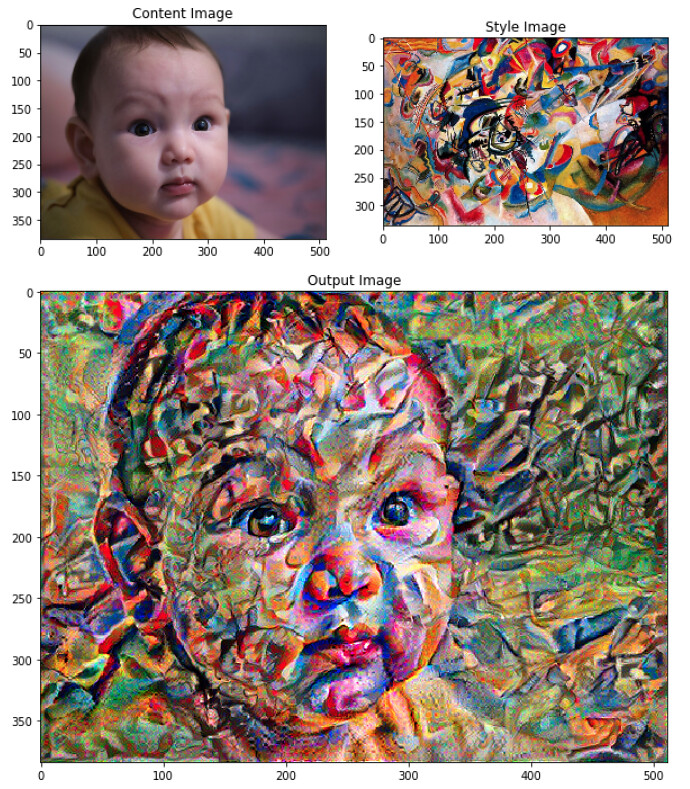
\includegraphics[width=60mm]{baby.jpeg}
    \end{center}
\end{frame}

\begin{frame}
		\frametitle{Key Finding}
		The representations of content and style in the Convolutional Neural Network are seperable.
\end{frame}

\begin{frame}
		\frametitle{Technical Stack}
		\setbeamertemplate{itemize items}[ball]
		\begin{itemize}
		\item Keras 
        \item Tensorflow
		\item NumPy
		\item SciPy
        \item Matplotlib
		\item Flask  
		\end{itemize}
\end{frame}

\begin{frame}
		\frametitle{Status}
		\setbeamertemplate{itemize items}[ball]
		\begin{itemize}
		\item Read the research paper.
		\item Completed the implementation of model.
        \item Working on website.
		\item Read the research paper.
		\end{itemize}
\end{frame}

\begin{frame}
		\frametitle{Learnings}
		\setbeamertemplate{itemize items}[ball]
        \begin{itemize}
		\item Learned to work with Version Control System conveniently.
		\item Learned to make presentation using Beamer.
		\item Studied about CNN.
        \item Learned HTML, CSS and JavaScript.
		\end{itemize}
\end{frame}

\begin{frame}
		\frametitle{Difficulties}
		\setbeamertemplate{itemize items}[ball]
        \begin{itemize}

				\item The program is taking lot of time to output stylized image.
                \item Allocating space for user image.
		\end{itemize}
\end{frame}

\begin{frame}
    \begin{center}  
       \Huge Thank You!
    \end{center}
\end{frame}

\end{document}
